\documentclass{article}

\usepackage{graphicx}
\usepackage[hidelinks]{hyperref}
\usepackage{geometry}
\usepackage{amsmath}
\usepackage{listings}
\usepackage{wrapfig}

\geometry{
 a4paper,
 left=20mm,
 right=20mm,
 top=20mm,
 bottom=25mm,
}

\begin{document}

\begin{titlepage}
\begin{center}
\vspace*{1cm}
            
\Huge
\textbf{Midterm Project}
            
\vspace{1cm}

\Large
\text{Due: Sunday, October 27, 2024}

\vspace{2cm}

\text{\texttt{Brian High}} \\
\text{\texttt{Thomas Hynes}} \\
\text{\texttt{Jeremy Middleman}} \\
\text{\texttt{Andrei Phelps}} \\
\text{\texttt{Wayne Rudnick}} \\

\vspace{2cm}

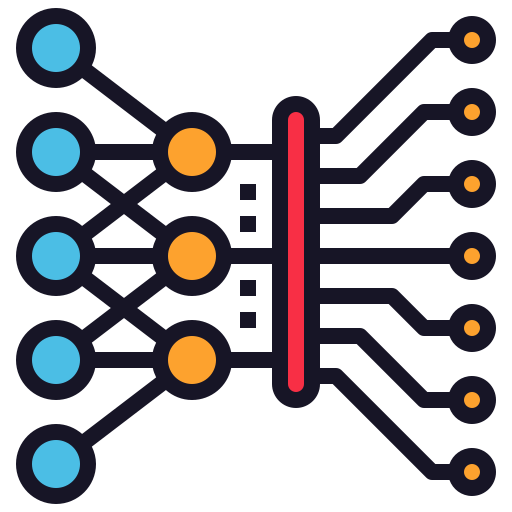
\includegraphics[scale=0.25]{figs/icon.png}\\[0.5cm]

\vspace{9cm}

\textbf{CS 491/591: Neural Networks} \\

\end{center}
\end{titlepage}
\newpage

\section{Feedforward Neural Network} 

The data structures that we used in order to make up our Feedforward Neural Network included

\subsubsection{\textbf{Layers}}
 Layers are stored as lists of layer objects containing 

\section{Backpropagation}
Backpropagation computes the error gradients for each layer and updates weights according to these gradients. In order to do this, we most propagate the error backwards through the network.


\section{Testing and Results}

\subsection{Simple Regression}

\subsection{Data Driven Model}
I ran a test based off of the ode specified in the assignment (x1 = x2,  ̇x2 = −x1 + (1 − x22)x2 and the ode that came with the Vanderpol file ([x[1], -x[0] + (1 - x[0]**2)*x[1]]). I did this because the ode specified in the assignment looked slightly different and I wanted to cover both bases in case one was perefed over the other.

Image from the ode specified in the assignment document (800 epochs): 

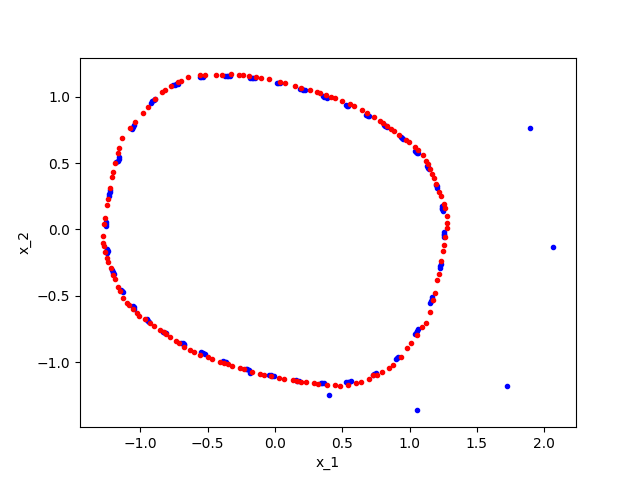
\includegraphics[scale=1]{figs/800AssignmentODE.png}\\[0.5cm]

\vspace{9cm}

Image from the Vanderpol file (800 epochs): 

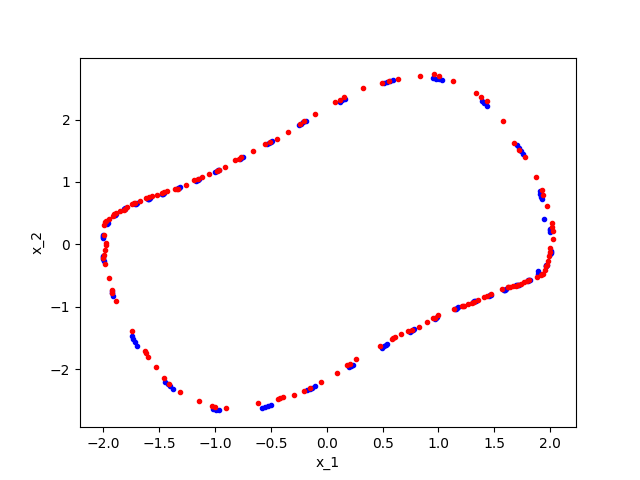
\includegraphics[scale=1]{figs/800VanderpolODE.png}\\[0.5cm]

\vspace{9cm}

\subsection{Handwriting Numbers}

\section{Individual Contributions}

\subsection{Brian High}
\begin{itemize}
    \item[1)]
\end{itemize}

\subsection{Thomas Hynes}
\begin{itemize}
    \item[1)]
\end{itemize}

\subsection{Jeremy Middleman}
\begin{itemize}
    \item[1)]
\end{itemize}

\subsection{Andrei Phelps}
\begin{itemize}
    \item[1)]
\end{itemize}

\subsection{Wayne Rudnick}
\begin{itemize}
    \item[1)]
\end{itemize}

\end{document}
